\section{Prerequisites}

This course uses many concepts from prerequisite courses, particularly those from calculus and circuits. While we assume you know this material, the following sections offer a review of the most pertinent and establish some notation. If you have trouble with any of them seek assistance -- the sooner the better.

\subsection*{Complex Numbers}

Complex numbers are used extensively throughout the course. You need to be very adept at manipulating them.

\subsubsection*{The Number System}

By way of review and to motivate the discussion of complext numbers, recall the following basic facts.

\begin{itemize}
\item The \emph{Natural Numbers} $\mathbb{N}$ are the positive integers $1,2,3,4,\cdots$. Given two natual numbers $a$ and $b$ the sum $a+b$ and the product $a\,b$ are also natural numbers, that is the set of natural numbers is \emph{closed} under addition and multiplication.

\item Solving equations of the form $x + a = b$ for any natural numbers $a,b$ requires the introduction of the negative integers $\cdots, -4, -3, -2 -1$ and $0$. These plus the natural numbers give the \emph{integers}  $\mathbb{Z}$. Note $\mathbb{N} \subset \mathbb{Z}$. Zero ($0$) is called the identity element with respect to addition, while $1$ is the identity with respect to multiplication, that is $a+0 = a$ and $ a \cdot 1 = a$. The \emph{inverse} of an integer $a$ is $-a$, such that thier sum gives the identity for addition, i.e. $a + -a = 0$.

\item The \emph{rational numbers} $\mathbb{Q}$ are of the form $\frac{b}{a}$ for integers $a,b$ with $a \neq 0$. They solve problems of the form $ax=b$ and provide the inverse for multiplication since $\frac{1}{a} \cdot a = 1$. Note $\mathbb{Z} \subset \mathbb{Q}$

\item The \emph{irrational numbers} are those that cannot be written as a rational number, for example $\sqrt{2} = 1.414\ldots$ and $\pi = 3.14159\ldots$

\item The union of the rational and irrational numbers give the \emph{real numbers} denoted $\mathbb{R}$.
\end{itemize}

Graphically the numbers and thier ordering can be expressed using the number line:

\begin{center}
  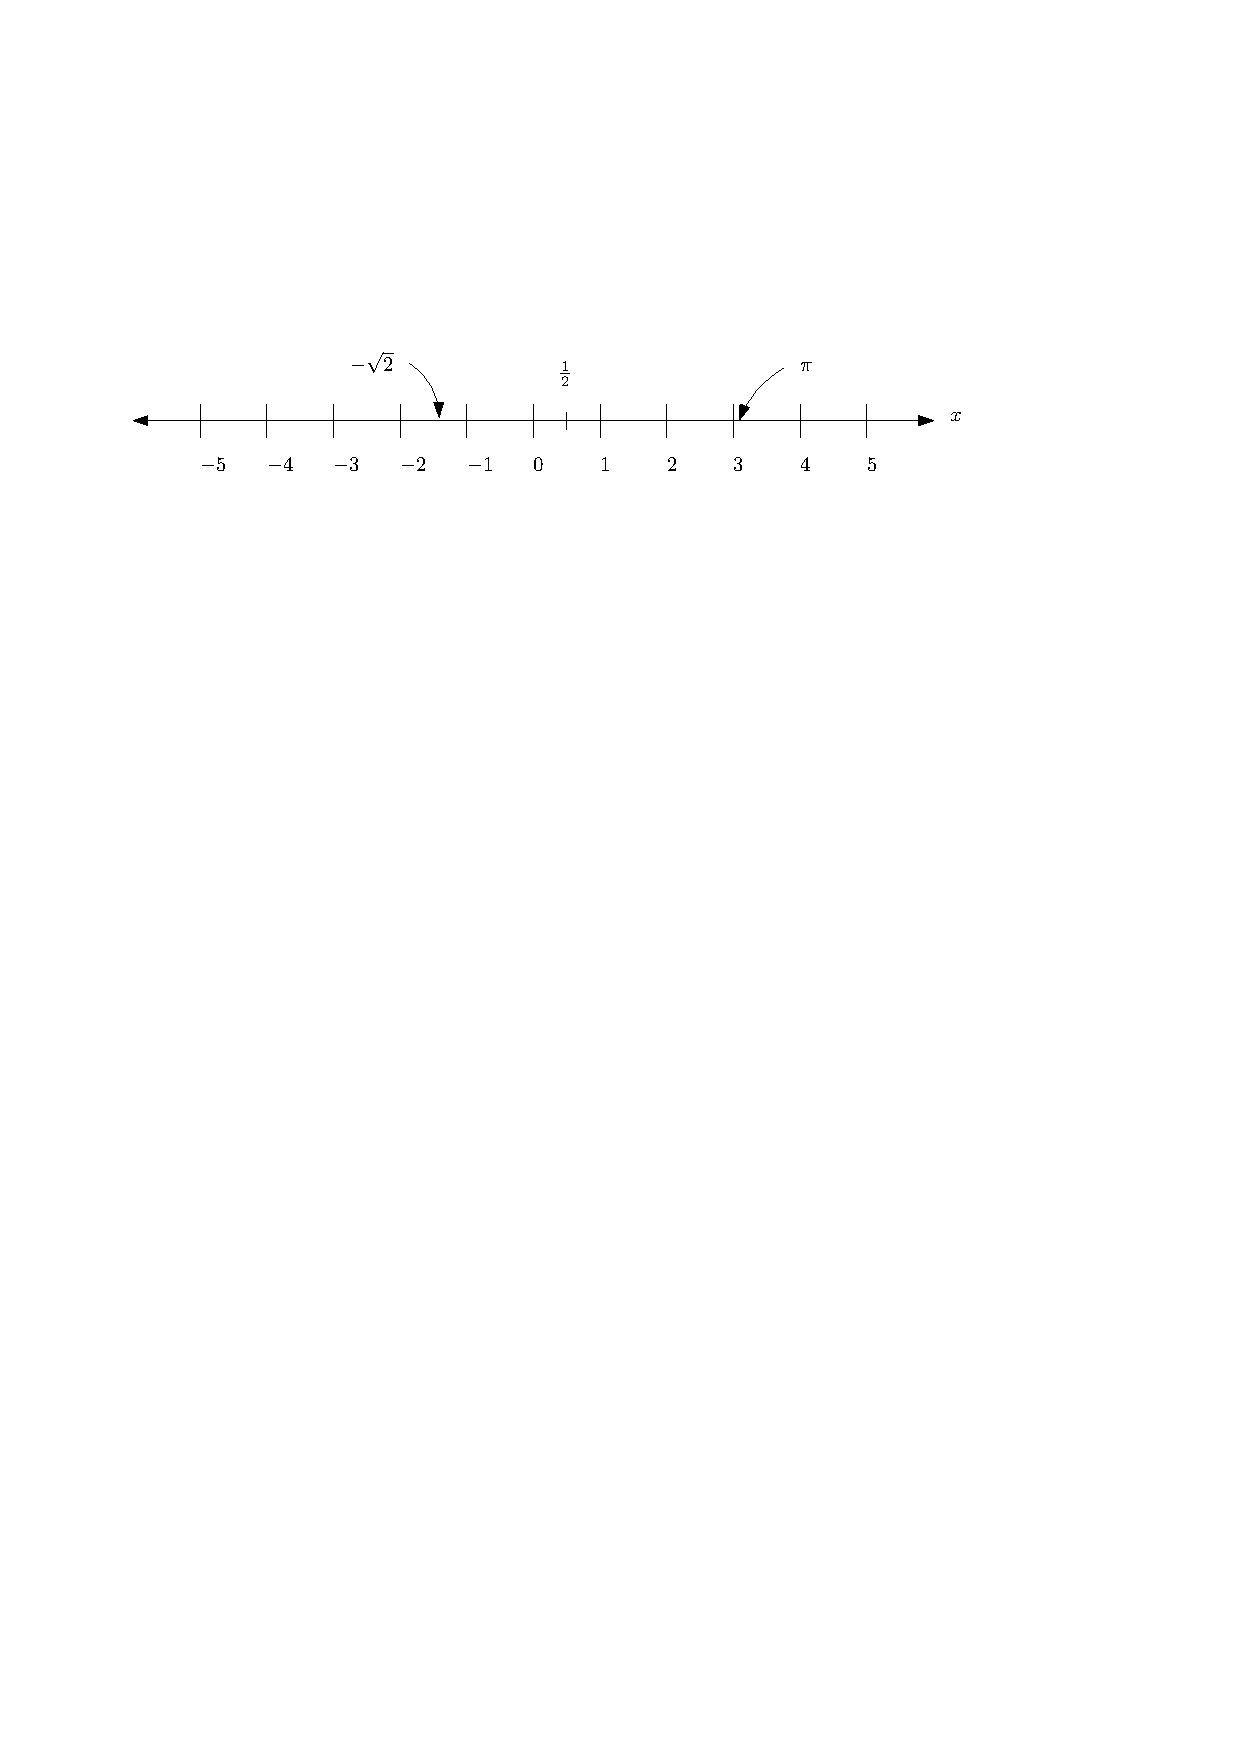
\includegraphics[scale=1]{graphics/number-line.pdf}
\end{center}

\subsubsection*{Complex numbers as extension of reals}

Continuing the pattern of the basic number system we can ask what are solutions of equations of the form $x^2+a = 0$ or $x^2 + 2ax +a^2 + b^2 = 0$ for $a,b \in \mathbb{R}$ ? As above, finding such solutions requires moving to a larger set of numbers, the \emph{complex numbers} denoted $\mathbb{C}$.

A complex variable $z\in\mathbb{C}$ can be written as $z = a + j\, b$ for $a,b\in\mathbb{R}$, where $j$ is the imaginary unit and $j^2 = -1$. Note in mathematics the imaginary unit is denoted $i$; this difference is purely historical. 

\begin{itemize}
\item the \emph{real part} $\Re(z) = \text{Re}(z) = a$
\item the \emph{imaginary part} $\Im(z) = \text{Im}(z) = b$
\item two complex numbers $z_1, z_2\in \mathbb{C}$ are equal if $\text{Re}(z_1) = \text{Re}(z_2)$ and $\text{Im}(z_1) = \text{Im}(z_2)$
\item $\mathbb{R} \subset \mathbb{C}$, when $b = 0$ and we say that the number is purely real
\item if $a = 0$ we say the number is purely imaginary
\item the \emph{complex conjugate} of $z = a + jb$ is $z^* = a - jb$.
\end{itemize}

\subsubsection*{Operations}


\subsubsection*{Absolute Value (Magnitude)}

\subsubsection*{Complex numbers as ordered pair}

\subsubsection*{Basic properties}

\begin{itemize}
\item equality
\item sum
\item product
\item closure
\item communative law of addition and multiplication
\item associative law of addition and multiplication
\item idenity elements 0 and 1
\item inverse -z and 1/z
\end{itemize}
\subsubsection*{Graphical representation of complex numbers}

TODO: Visualization of multiplication by j.

\subsubsection*{Polar representation of complex numbers, Magnitude an Phase}

\subsubsection*{De Moivre's Theorem}

\subsubsection*{Roots and powers of complex numbers}

\subsubsection*{Euler's formula}

\subsubsection*{Complex numbers as roots of polynomial equations}

\subsubsection*{The nth roots of unity}

\subsubsection*{Vector interpretation of complex numbers}

\subsection*{Calculus}

\subsubsection*{Functions}

\begin{itemize}
\item $f:\mathbb{R}\mapsto\mathbb{R}$
\item $f:\mathbb{R}\mapsto\mathbb{C}$
\end{itemize}

\subsubsection*{Review derivative}

\subsubsection*{Review Reimann integral}

Complex integrals?

\subsubsection*{Numerical approximations?}

\subsection*{Complex valued functions}

\subsubsection*{functions from reals to complex}

\subsubsection*{derivatives of such functions}

\subsubsection*{integrals of such functions}

\subsubsection*{Magnitude and Phase representation of such functions}

\subsection*{Differential Equations}

\subsubsection*{linear, constant-coefficient differential equations, homogeneous and particular solutions}

\subsection*{Circuits}

\subsubsection*{KVL}

\subsubsection*{KCL}

\subsubsection*{Ideal OpAmps}

\subsubsection*{from circuit to differential equation}

\subsubsection*{using LiaB and building/measuring circuits}

\subsection*{Programming}

\subsubsection*{plotting and vizualization with Matlab/Python/Julia}

\subsubsection*{Computation with C or C++}

\subsection*{Digitial Systems}

\subsubsection*{binary representation of integers vs floating point}

\subsubsection*{shift registers}

\subsubsection*{adders and multipliers}

\subsubsection*{FPGAs?}
